% Options for packages loaded elsewhere
\PassOptionsToPackage{unicode}{hyperref}
\PassOptionsToPackage{hyphens}{url}
\PassOptionsToPackage{dvipsnames,svgnames,x11names}{xcolor}
%
\documentclass[
  12pt]{article}

\usepackage{amsmath,amssymb}
\usepackage{iftex}
\ifPDFTeX
  \usepackage[T1]{fontenc}
  \usepackage[utf8]{inputenc}
  \usepackage{textcomp} % provide euro and other symbols
\else % if luatex or xetex
  \usepackage{unicode-math}
  \defaultfontfeatures{Scale=MatchLowercase}
  \defaultfontfeatures[\rmfamily]{Ligatures=TeX,Scale=1}
\fi
\usepackage{lmodern}
\ifPDFTeX\else  
    % xetex/luatex font selection
\fi
% Use upquote if available, for straight quotes in verbatim environments
\IfFileExists{upquote.sty}{\usepackage{upquote}}{}
\IfFileExists{microtype.sty}{% use microtype if available
  \usepackage[]{microtype}
  \UseMicrotypeSet[protrusion]{basicmath} % disable protrusion for tt fonts
}{}
\makeatletter
\@ifundefined{KOMAClassName}{% if non-KOMA class
  \IfFileExists{parskip.sty}{%
    \usepackage{parskip}
  }{% else
    \setlength{\parindent}{0pt}
    \setlength{\parskip}{6pt plus 2pt minus 1pt}}
}{% if KOMA class
  \KOMAoptions{parskip=half}}
\makeatother
\usepackage{xcolor}
\setlength{\emergencystretch}{3em} % prevent overfull lines
\setcounter{secnumdepth}{5}
% Make \paragraph and \subparagraph free-standing
\makeatletter
\ifx\paragraph\undefined\else
  \let\oldparagraph\paragraph
  \renewcommand{\paragraph}{
    \@ifstar
      \xxxParagraphStar
      \xxxParagraphNoStar
  }
  \newcommand{\xxxParagraphStar}[1]{\oldparagraph*{#1}\mbox{}}
  \newcommand{\xxxParagraphNoStar}[1]{\oldparagraph{#1}\mbox{}}
\fi
\ifx\subparagraph\undefined\else
  \let\oldsubparagraph\subparagraph
  \renewcommand{\subparagraph}{
    \@ifstar
      \xxxSubParagraphStar
      \xxxSubParagraphNoStar
  }
  \newcommand{\xxxSubParagraphStar}[1]{\oldsubparagraph*{#1}\mbox{}}
  \newcommand{\xxxSubParagraphNoStar}[1]{\oldsubparagraph{#1}\mbox{}}
\fi
\makeatother


\providecommand{\tightlist}{%
  \setlength{\itemsep}{0pt}\setlength{\parskip}{0pt}}\usepackage{longtable,booktabs,array}
\usepackage{calc} % for calculating minipage widths
% Correct order of tables after \paragraph or \subparagraph
\usepackage{etoolbox}
\makeatletter
\patchcmd\longtable{\par}{\if@noskipsec\mbox{}\fi\par}{}{}
\makeatother
% Allow footnotes in longtable head/foot
\IfFileExists{footnotehyper.sty}{\usepackage{footnotehyper}}{\usepackage{footnote}}
\makesavenoteenv{longtable}
\usepackage{graphicx}
\makeatletter
\def\maxwidth{\ifdim\Gin@nat@width>\linewidth\linewidth\else\Gin@nat@width\fi}
\def\maxheight{\ifdim\Gin@nat@height>\textheight\textheight\else\Gin@nat@height\fi}
\makeatother
% Scale images if necessary, so that they will not overflow the page
% margins by default, and it is still possible to overwrite the defaults
% using explicit options in \includegraphics[width, height, ...]{}
\setkeys{Gin}{width=\maxwidth,height=\maxheight,keepaspectratio}
% Set default figure placement to htbp
\makeatletter
\def\fps@figure{htbp}
\makeatother

\addtolength{\oddsidemargin}{-.5in}%
\addtolength{\evensidemargin}{-1in}%
\addtolength{\textwidth}{1in}%
\addtolength{\textheight}{1.7in}%
\addtolength{\topmargin}{-1in}%
\makeatletter
\@ifpackageloaded{caption}{}{\usepackage{caption}}
\AtBeginDocument{%
\ifdefined\contentsname
  \renewcommand*\contentsname{Table of contents}
\else
  \newcommand\contentsname{Table of contents}
\fi
\ifdefined\listfigurename
  \renewcommand*\listfigurename{List of Figures}
\else
  \newcommand\listfigurename{List of Figures}
\fi
\ifdefined\listtablename
  \renewcommand*\listtablename{List of Tables}
\else
  \newcommand\listtablename{List of Tables}
\fi
\ifdefined\figurename
  \renewcommand*\figurename{Figure}
\else
  \newcommand\figurename{Figure}
\fi
\ifdefined\tablename
  \renewcommand*\tablename{Table}
\else
  \newcommand\tablename{Table}
\fi
}
\@ifpackageloaded{float}{}{\usepackage{float}}
\floatstyle{ruled}
\@ifundefined{c@chapter}{\newfloat{codelisting}{h}{lop}}{\newfloat{codelisting}{h}{lop}[chapter]}
\floatname{codelisting}{Listing}
\newcommand*\listoflistings{\listof{codelisting}{List of Listings}}
\makeatother
\makeatletter
\makeatother
\makeatletter
\@ifpackageloaded{caption}{}{\usepackage{caption}}
\@ifpackageloaded{subcaption}{}{\usepackage{subcaption}}
\makeatother

\ifLuaTeX
  \usepackage{selnolig}  % disable illegal ligatures
\fi
\usepackage[]{natbib}
\bibliographystyle{agsm}
\usepackage{bookmark}

\IfFileExists{xurl.sty}{\usepackage{xurl}}{} % add URL line breaks if available
\urlstyle{same} % disable monospaced font for URLs
\hypersetup{
  pdftitle={DOGE Days on Reddit: Decoding Public Sentiment in a Federal Shakeup},
  pdfauthor={Kevin Linares; Felix Baez-Santiago; Aria Lu; Gloria Zhou},
  pdfkeywords={Reddit, Federal Government, DOGE},
  colorlinks=true,
  linkcolor={blue},
  filecolor={Maroon},
  citecolor={Blue},
  urlcolor={Blue},
  pdfcreator={LaTeX via pandoc}}



\begin{document}


\def\spacingset#1{\renewcommand{\baselinestretch}%
{#1}\small\normalsize} \spacingset{1}


%%%%%%%%%%%%%%%%%%%%%%%%%%%%%%%%%%%%%%%%%%%%%%%%%%%%%%%%%%%%%%%%%%%%%%%%%%%%%%

\date{March 21, 2025}
\title{\bf DOGE Days on Reddit: Decoding Public Sentiment in a Federal
Shakeup}
\author{
Kevin Linares\\
University of Maryland\\
and\\Felix Baez-Santiago\\
and\\Aria Lu\\
and\\Gloria Zhou\\
University of Michigan\\
}
\maketitle

\bigskip
\bigskip
\begin{abstract}
This study explores the impact of the Department of Government
Efficiency (DOGE)'s federal workforce reductions, known as reduction in
force (RIF), on public sentiment, utilizing Reddit as a data source. We
scraped the Reddit API from March 2nd to March 10th resulting in 557
unique posts with 12,553 comments from subreddits related to DOGE's
approach to the RIF. Our exploratory analysis captures peaks in the
number of posts/comments following major news event coverage related to
the RIF, highlighting the utility of social media for understanding
public perception of policy impacts. Our text analysis reveals a
saliency on community with words such as people, employees, service,
public, workers, and care being top words in both posts and comments.
Moreover, a team of researchers coded a random subset of comments for
public sentiment and found that only a quarter approved of DOGE's
actions towards the RIF.
\end{abstract}

\noindent%
{\it Keywords:} Reddit, Federal Government, DOGE
\vfill

\newpage
\spacingset{1.9} % DON'T change the spacing!


\section{Introduction}\label{sec-intro}

Since its inception in January 2025, the Department of Government
Efficiency (DOGE) has implemented significant reductions in the federal
workforce, resulting in the separation of over 200,000 employees, in
alignment with the new administration's campaign promises. These
reductions have generated widespread concern and anxiety among federal
workers regarding their job security and mental well-being. Reports
indicate that DOGE's methods have raised questions about adherence to
established internal policies. The ongoing debate surrounding DOGE's
impact on federal worker perceptions of job security necessitates a
thorough examination. This study proposes that Reddit, as a platform for
public discourse, provides researchers with valuable insights into
real-time reactions and discussions among federal workers on this topic.
Furthermore, this research aims to capture a range of public sentiments,
including both critical and supportive perspectives, regarding DOGE's
workforce reduction efforts.

\section{Methods}\label{sec-meth}

\emph{Search Terms}. Our initial Reddit API scrape facilitated the
development of a targeted keyword search strategy for this research.
This iterative process resulted in the selection of eight keywords (see
Table 1). We excluded keywords deemed vague or overly broad, such as
`Elon Musk' or `drain the swamp.' Additionally, we observed that certain
keywords yielded a high volume of irrelevant posts. For example, `policy
changes' returned numerous discussions unrelated to government workforce
reductions. Similarly, `DOGE' produced results related to DOGEcoin,
which is outside the scope of this study. Therefore, we meticulously
examined the subreddits identified in our initial scrape and selected
those containing relevant discussions. To ensure a balanced
representation of viewpoints, we included subreddits with conservative
perspectives, such as `neoliberal' and `AskConservatives,' while
avoiding subreddits focused on specific agencies like `NIH' or `CDC,'
which could skew the data. In total, we selected 19 subreddits (see
Appendix A) and utilized eight keywords, resulting in 152 unique keyword
and subreddit combinations for our data collection.

\begin{longtable}[]{@{}l@{}}
\caption{List of keywords related to topic}\tabularnewline
\toprule\noalign{}
search\_term \\
\midrule\noalign{}
\endfirsthead
\toprule\noalign{}
search\_term \\
\midrule\noalign{}
\endhead
\bottomrule\noalign{}
\endlastfoot
DOGE \\
Department of Government Efficiency \\
wasteful spending \\
government waste \\
government fraud \\
reduction in force \\
rif \\
fork in the road \\
\end{longtable}

\emph{Analytic Plan}. We collected data from the Reddit API hourly, from
March 2nd through the 10th, by scraping each combination of our eight
keywords and 19 subreddits, resulting in 152 API requests per hour.
Reddit API rate limits were managed by implementing a sleep timer
between requests. Raw data from new Reddit posts were entered into a
data table without initial processing. Following the data collection
period, the raw dataset contained 643 posts. Each row in the data table
represented a single post, and the columns included the post's date and
time, title, text, subreddit, comment count, URL, and the search term
used for collection. Duplicate posts, which occurred when multiple
keywords matched the same post, were removed. Post text was cleaned by
removing weblinks and converting special characters, such as the at
sign, to the word `at.' The date column was converted to a date class
variable, and the day of the week and time of day were extracted for
analysis. After cleaning, the dataset consisted of 557 posts.

A preliminary review of the posts revealed that many were factual
statements, questions, or reposted news articles and videos, which were
not suitable for sentiment coding. Therefore, we also scraped the
comments associated with each post. This resulted in 12,553 comments
after processing, including information on score, up/down votes, and
date/time. Comments containing only weblinks, videos, or images were
removed. A review of the comments revealed more opinionated statements
and reactions. We then randomly selected 400 comments (without
replacement) and assigned them to four graduate students for coding,
categorizing each comment as favoring, opposing, or neutral towards
DOGE's approach to federal workforce reductions.

\section{Results}\label{results}

\emph{Post and Comment Trends}

We show the number of posts pre/post processing by day in Figure 1
during the timeframe that we collected these data. There appears to be a
noticeable peak in activity during the middle of the week. However, we
don't have enough data across weeks to conclusively say it is due to the
day of the week itself. It is more likely that these spikes are linked
to specific events that occurred on those days, which sparked
conversations. The two peaks in our graph could be attributed to two
major news stories. On March 5th, Elon Musk made a statement about
wanting to ``save Western civilization from empathy,'' and on March 6th,
there were reports that President Trump was limiting Musk's authority
due to backlash over cuts to DOGE. These events likely had a significant
impact on the volume of Reddit posts related to Elon Musk and DOGE,
driving the observed spikes in activity.

On March 3rd, news outlets started reporting that DOGE was claiming
\$105 billion dollars in savings from cutting ``wasteful'' spending by
layoffs and cutting foreign aid. This amount is controversial since
since the receipts shown on their site only amount to less than
\href{https://abcnews.go.com/US/doge-website-now-saved-105-billion-backtracked-earlier/story?id=119408347}{\$9.6
billion}. This could have prompted Reddit users to take to subreddits
and provide their opinion or thoughts on this matter.

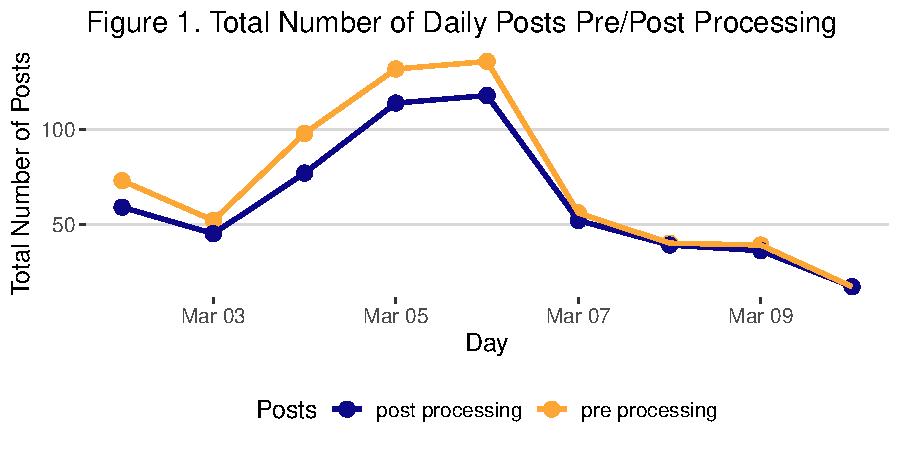
\includegraphics{paper_files/figure-pdf/unnamed-chunk-3-1.pdf}

We see a peak in the comments in Figure 2 on March 6th, which was a
Thursday, and perhaps in anticipation of DOGE policies that often are
released on Friday morning and have come to be known as
``\href{https://smotus.substack.com/p/friday-night-musk-acre}{Musk-acre
Friday}.''

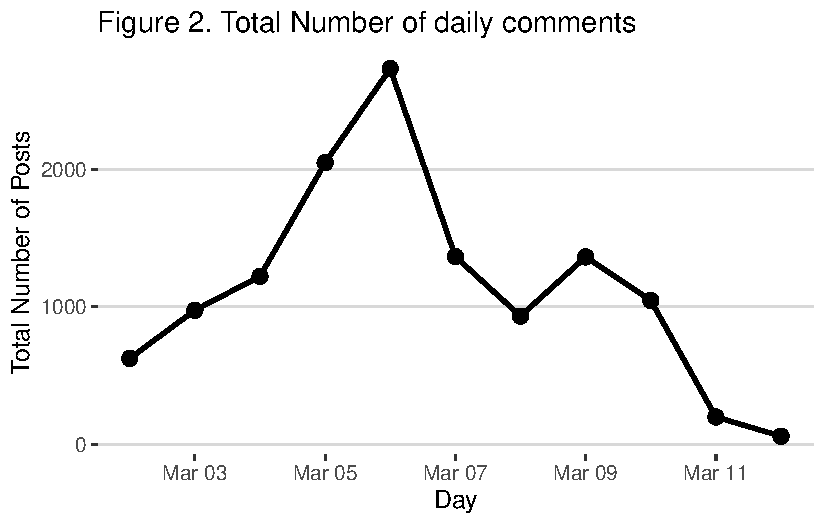
\includegraphics{paper_files/figure-pdf/unnamed-chunk-4-1.pdf}

\emph{Word Frequency}

Most posts occur during the early morning, noon, and afternoon hours
(see Figure 3). The highest peak is around lunchtime, likely due to
people posting during their lunch break. There is also significant
activity in the afternoon, evening, and early morning. It is possible
that people have more time in the evenings allowing them to be more
likely to post on Reddit. The fewest posts are seen in the morning,
which makes sense as people are typically getting ready for work,
commuting, or sleeping in. The trend for comments (see Figure 3) mirrors
that of posts. This makes sense because people are likely using Reddit
at similar times for both posting and commenting. However, the volume of
comments is much higher than the number of posts, as each post receives
many comments from different users.

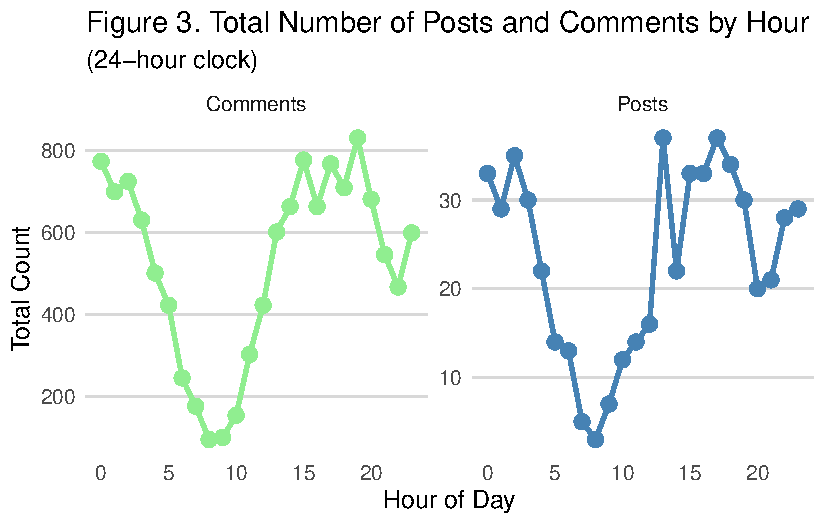
\includegraphics{paper_files/figure-pdf/unnamed-chunk-5-1.pdf}

The graphs below (Figure 4) show the most frequent words used in both
Reddit posts and their comment sections while excluding our keyword
search terms. These words were identified by tokenizing the text and
removing stop words, then counting the occurrences of the most common
terms. The removal of stop words allowed us to focus on contextual words
in the posts/comments rather than common words like ``the'' and ``and''
that are not useful in these types of analysis. Examining this visual
reveals that in posts the current president's name is the top word.
However, in both posts and comments, there appears to be an emerging
theme of community as words like people, employees, service, care, jobs,
and public are also top words. This highlights the focus of the
community on these key themes, reflecting the ongoing conversations and
interests of Reddit users within this context.

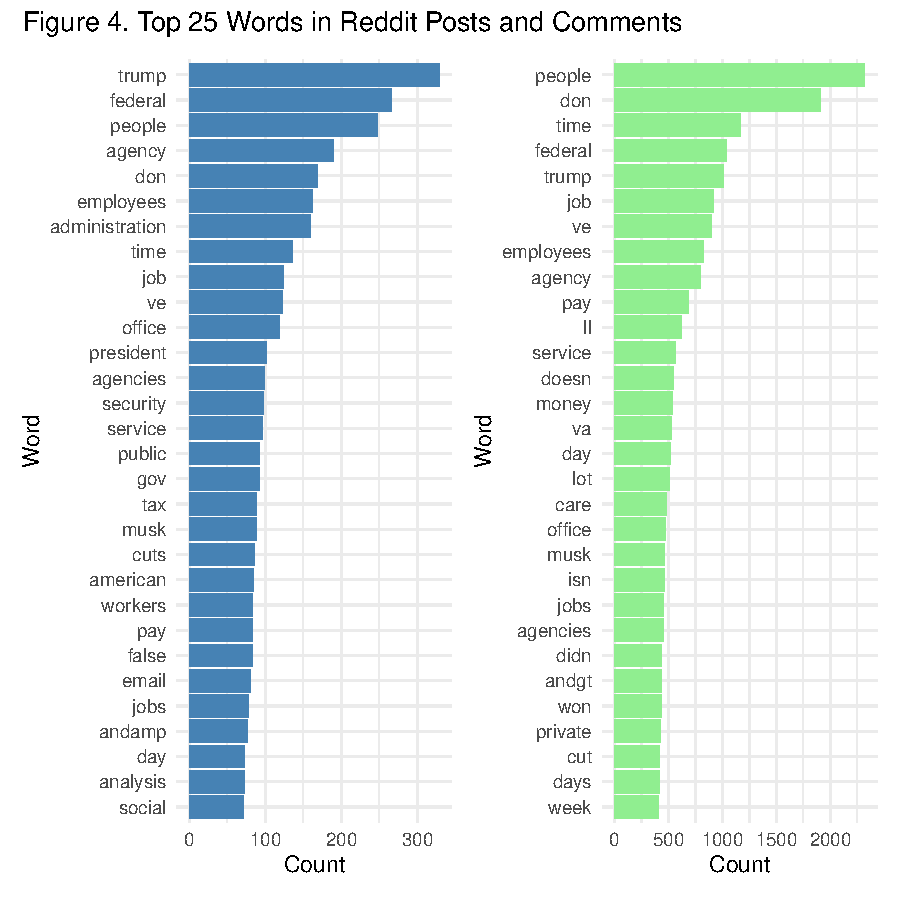
\includegraphics{paper_files/figure-pdf/unnamed-chunk-6-1.pdf}

\emph{Coding Comments}

We randomly selected and coded 400 comments from the Reddit posts. Table
2 shows the distribution of favorability coding for these comments.
Among the 400 comments, the majority (217) expressed opposition to
DOGE's approach to reducing the federal workforce, while 110 were
supportive, and 73 remained neutral. A large number of comments (12,153)
were not coded, as their content was not relevant for favorability
assessment.

\begin{longtable}[]{@{}lr@{}}
\caption{Distribution of favorability coding for 400
comments}\tabularnewline
\toprule\noalign{}
outcome & Total \\
\midrule\noalign{}
\endfirsthead
\toprule\noalign{}
outcome & Total \\
\midrule\noalign{}
\endhead
\bottomrule\noalign{}
\endlastfoot
Not Coded & 12153 \\
favor & 110 \\
neutral & 73 \\
oppose & 217 \\
\end{longtable}

\section{Conclusion}\label{conclusion}

In this study, we explored the impact of the DOGE's actions towards the
reduction in force impacting federal workers' perceptions of job
security, using Reddit as a platform to analyze public discourse. In
examining Reddit posts and comments related to DOGE's workforce
reduction policies, we gained valuable insights into the sentiments of
both federal workers and the broader public. Our findings indicate that
these discussions are heavily influenced by political events and
high-profile figures, such as President Trump and Elon Musk, with
particular attention given to DOGE's controversial cost-cutting
measures. Through the analysis of both posts and comments, we captured a
wide range of reactions, with the majority being strongly opposed to
DOGE's approach. The frequent mention of terms related to the
administration underscores the community's focus on government policies
and the emotional responses these issues generate.

In terms of favorability, the distribution of comments revealed that 217
out of 400 were opposed to DOGE's approach, 110 were supportive, and 73
were neutral. Additionally, patterns in post volume, especially peaks
during significant news events, highlight the dynamic nature of these
discussions, providing insights into the timing and public reactions to
key policy decisions. While our study provides a snapshot of Reddit
discussions during a specific period, the findings demonstrate the value
of social media platforms like Reddit in capturing public sentiment on
contemporary political and policy issues. However, it is important to
note that Reddit may not fully represent the broader population's views,
as the platform tends to skew younger and more politically engaged,
potentially limiting the generalizability of these findings.

The use of sentiment analysis on social media presents challenges, as it
can be influenced by sarcasm, humor, or polarized language, which might
affect the accuracy of sentiment classification. Therefore, our research
team hand coded a subset of comments, yet inter-rater reliability was
not estimated. The specific subreddits analyzed, while designed to
capture diverse perspectives, may still over-represent certain political
or ideological viewpoints. Moreover, the relatively short timeframe of
this analysis---spanning only March 2nd to March 10th---means that we
may not have captured long-term trends or shifts in sentiment as the
DOGE policies unfold. Future research could address these limitations by
expanding the data collection to other platforms or a longer timeframe
and by incorporating demographic data to better understand the views of
different Reddit user groups.

\newpage

\section{Appendix}\label{appendix}

We examined almost 100 subreddit posts while paying attention to the
post topics and determined which ones were related to our topic. We also
included right leaning subreddits to attempt to capture a balanced
public sentiment on the topic. The following is our final list of
subreddits that we scraped from.

\begin{longtable}[]{@{}l@{}}
\caption{List of subreddits relevant to the topic of
DOGE}\tabularnewline
\toprule\noalign{}
subreddit \\
\midrule\noalign{}
\endfirsthead
\toprule\noalign{}
subreddit \\
\midrule\noalign{}
\endhead
\bottomrule\noalign{}
\endlastfoot
50501 \\
fednews \\
neoliberal \\
FedEmployees \\
WhatTrumpHasDone \\
Whistleblowers \\
economy \\
PoliticalOpinions \\
Trumpvirus \\
Virginia \\
Libertarian \\
AskTrumpSupporters \\
Askpolitics \\
Conservative \\
VeteransAffairs \\
economicCollapse \\
feddiscussion \\
maryland \\
govfire \\
\end{longtable}




\end{document}
